
%(BEGIN_QUESTION)
% Copyright 2011, Tony R. Kuphaldt, released under the Creative Commons Attribution License (v 1.0)
% This means you may do almost anything with this work of mine, so long as you give me proper credit

Weirs and flumes are frequently equipped with stilling wells to provide a ``quiet'' liquid height for an instrument to measure.  In this case a {\it displacer} is being used to measure the height of liquid inside the stilling well:

$$\includegraphics[width=15.5cm]{i03423x01.eps}$$

Suppose the flow transmitter (FT) sensing displacer buoyancy needs to output a signal that is linear with flow.  You know that weirs and flumes are very non-linear, and so a normal displacer will simply report the height of water rather than the linearized flow rate of water through the channel.

\vskip 10pt

One solution to this characterization problem is to re-shape the displacer to perform this linearization for us.  Assuming the use of a Cippoletti weir as the flow element in this system (flow equation shown below), qualitatively sketch the shape of a displacer necessary to make the flow transmitter (FT) output a signal linearly proportional to flow, explaining why this new shape is necessary.

$$Q = 3.367 L H^{1.5} \hbox{\hskip 20pt Flow equation for a Cippoletti weir}$$

\noindent
Where,

$Q$ = Volumetric flow rate (cubic feet per second -- CFS)

$L$ = Width of crest (feet)

$H$ = Liquid height above weir crest (feet)

\vskip 10pt


\vskip 50pt

\underbar{file i03423}
%(END_QUESTION)





%(BEGIN_ANSWER)

5 point for shape, 5 points for explanation:

$$\includegraphics[width=15.5cm]{i03423x02.eps}$$

The displacer needs to be tapered (skinny at bottom and wide at top) in order to characterize flow.  At low flow rates (low stilling well levels), small changes in water level only represent small changes in flow rate.  At high flow rates (high stilling well levels), the same small changes in water level represent much larger changes in flow rate.  Therefore, the displacer's cross-sectional area needs to be larger toward its top, so that larger increments of buoyant force will be generated for a given level change at the top than at the bottom. 

%(END_ANSWER)





%(BEGIN_NOTES)

{\bf This question is intended for exams only and not worksheets!}.

%(END_NOTES)

